\subsection{Equivalence Classes}
\label{ss_equiv}

We now introduce the concept of equivalence classes, as proposed by "Applegate et al."'s paper. This definition will allow us to give structure on the order of which columns and rows should be picked-up during an execution of MPUS in order to find an optimal SRRL.

\subsubsection{Definition and Properties.}
Given a pattern P, we define two rows or columns as being of the same equivalence class if and only if they are both of the same type (row or column) and their cells have the exact same colors in P, in the same order; that is, they are identical.

We will denote a column equivalence class in a pattern $P$ as being $C_{x}$ where $x$ is the number of black cells in the original pattern. Analogously, we will denote $R_{y}$ as being the row class with $y$ black cells in the original pattern. See Fig.~\ref{fig:equiv_classes_example} for an example of a pattern and its equivalence classes.
It follows from the monotocity property (Theorem
\ref{theorem_strip_rule_patterns}
in Subsection \ref{ss_monoton} of the Appendix)
 that all the columns in $C_x$ are identical in all
positions, for all $x$, and the same property holds for all the rows of $R_y$,
for all $y$.

\begin{figure}[h]
\centering
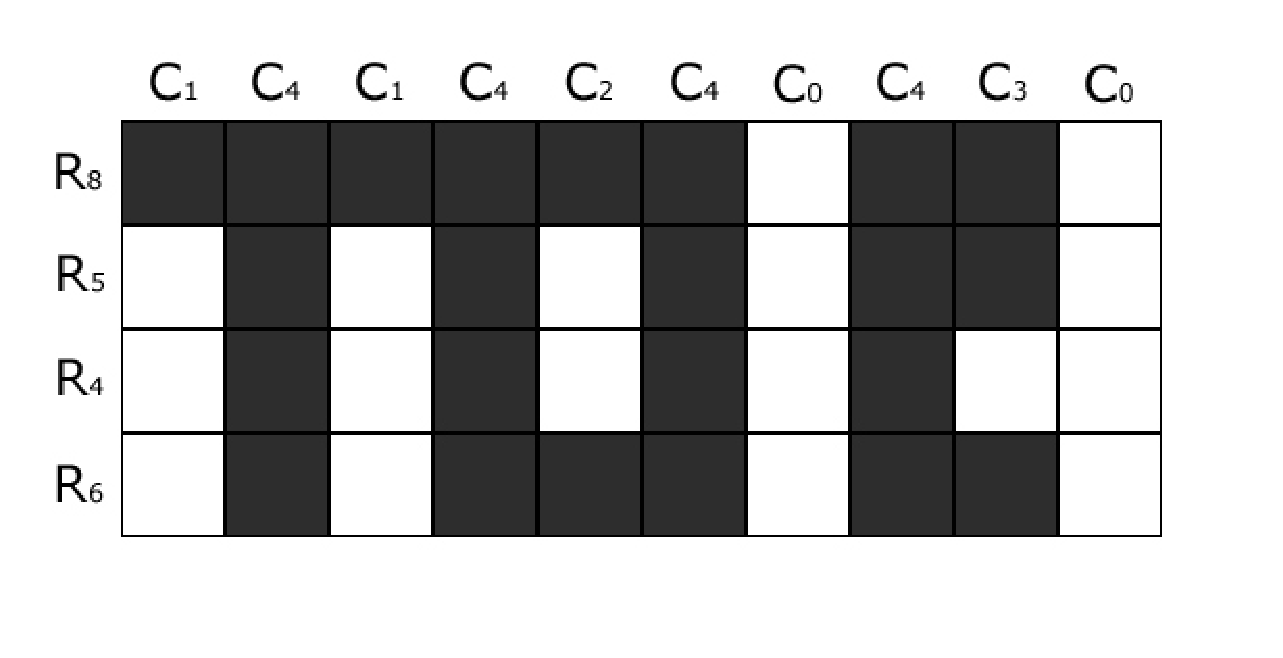
\includegraphics[height=5cm]{equiv_classes_example}
\caption{Equivalence classes of a black and white pattern P.}
\label{fig:equiv_classes_example}
\end{figure}

Note that every row and column belongs to exactly one equivalence class. Also, if two columns belong to a equivalence class in the beginning of the MPUS algorithm, they will remain of the same class until one of them is picked up
by the algorithm. This is since picking up other columns does not
change these two columns at all, while picking up rows modify these
two columns in exactly the same way. The same property holds for two
rows that belong to a equivalence class.

 %the very end of its execution. This will be proven later,
 %but the idea is that if any cell of row or column is removed,
 % the same cell will be removed for every member of its equivalence class.

We also define an equivalence class as being {\em active} during the execution of the MPUS algorithm if some member of that class is pseudo-monochromatic
but not all gray.

\subsubsection{Active Classes Properties.}
"Applegate et al."'s paper shows that during the execution of the MPUS algorithm on a black and white strip-rule pattern, there are always exactly two active classes at any given time.
The intuition on why this happens is that in order for a new class to become active, all the members of an old active class need to be picked up.
A formal proof of this property appears later in
Proposition \ref{t_active_classes} in the Appendix
(Subsection \ref{ss_classes});
this fact is also used in \cite{ACJKLW07}.
Also, the same proposition shows that
the two active classes are either a row and a column
class of the same color or both classes of the same kind (rows or columns),
 being one of each color.

\subsubsection{Embedded Rows and Columns.}
We can start improving the MPUS algorithm by introducing the concept described by "Applegate et al."'s paper as embedded rows and columns. This will allow us to pick up more rows and columns using the same number of rectangles.

First, we will define the concept of a embedded column or row at a given stage of the MPUS algorithm.
Given a point during the execution of the MPUS algorithm,
let $b$ be a column of an active equivalence class $B$.
Let $a_{1}$ be the first column to the left of $b$ that does not belong to $B$ and has not yet been picked up.
Similarly, let $a_{2}$ be the first column to the right of $b$ that does not belong to $B$ and has not yet been picked up.
We say that $b$ is {\em embedded}
 in equivalence class $A$ if both $a_{1}$ and $a_{2}$ belong to that class $A$. The definition is analogous for rows. Note that columns can be embedded only in column classes and rows only in row classes. See the three leftmost columns of Fig.~\ref{fig:embedment_example} for a simple example of a white column embedded in two black columns.

\begin{figure}[h]
\centering
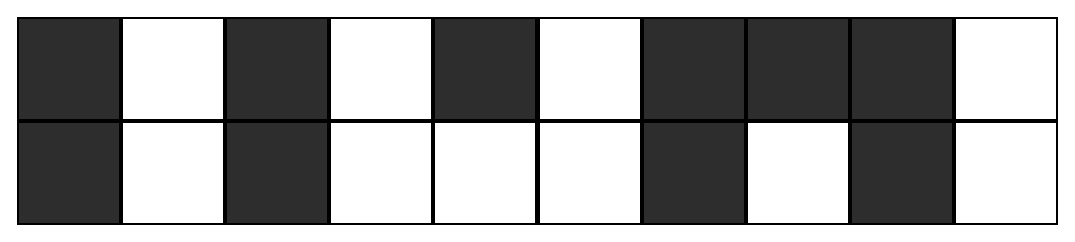
\includegraphics[width=10cm]{embedment_example}
\caption{Example of a pattern $P$ where some members of $C_{0}$ are embedded in some members of $C_{2}$.}
\label{fig:embedment_example}
\end{figure}

If during the execution of the MPUS algorithm we have the option to pick up two
column-blocks that embeds a set of columns of another class,
 we could pick up the two column-blocks that embeds the third one with
 two rectangles and then the embedded one, totaling three rectangles.
 However, it is better to pick the embedded block first with one rectangle,
and then pick the two blocks that were previously embedding with only one
rectangle, thus using a total of two rectangles for the same set of columns.
As an example, in Fig.~\ref{fig:embedment_example}, one cannot benefit
by picking up the first and the third column, when one can pick up
first the second column, followed by picking up the block of the first three
columns.

\subsubsection{Equivalence Classes Ordering.}
\label{ss_ordering}
As we pick up all the members of a column class, we change the rows of the pattern. Since the other columns remain intact, the new class to become active must be a row class. By using the same argument for row classes, we see that whenever we pick up all the members of a class, the next class to become active is of the opposite type.  This is formally proven in Proposition
\ref{theorem_pick_up_altertation} in the Appendix.
Also (same proposition), if we pick up all the members of an active class that was pseudo-monochromatic on a given color (for instance, black), the next class to become active needs to be of the opposite color (for instance, white). This happens because if it was of the same color, the other class would already have been active.

We can order the equivalence classes of both rows and columns in a given
 pattern $P$ by the number of black cells on it. In that ordering,
we can see (Proposition \ref{theorem_difference_is_class} in the Appendix)
that the all the rows that two consecutive column classes differ
 form exactly an equivalence class. This holds analogously for columns.
This implies (Proposition \ref{lemma_num_rows_col_differ_one} in the Appendix)
that the numbers of columns and rows classes differ
by at most one.  Using that information,
 we can set up the following ordering for the equivalence classes
(see also Proposition \ref{corollary_hierarchical_sequence} in the Appendix):

\begin{enumerate}

\item Start with the column class with only white cells. If such class does not exist, start with the row class with only black cells  (the existence of
this row class follows immediately from the monotonicity property -
Theorem \ref{theorem_strip_rule_patterns} in the Appendix).

\item Alternate columns and rows, putting the columns in ascending order of black cells and the rows in descending order of black cells.

\end{enumerate}

Let $C_{x_{0}}, C_{x_{1}}, \cdots, C_{x_{(N_{C}-1)}}, C_{x_{N_{C}}}$ be the ascending ordering of column classes by the number of black cells. Let $R_{y_{0}}, R_{y_{1}}, \cdots, R_{y_{(N_{R}-1)}}, R_{y_{N_{R}}}$ be the ascending ordering of row classes by the number of black cells. Using the rules above, we should get an ordering similar to $C_{x_{0}}, R_{y_{N_{R}}}, C_{x_{1}}, R_{y_{(N_{R}-1)}}, \cdots, R_{y_{1}}, C_{x_{(N_{C}-1)}}, R_{y_{0}}, C_{x_{N_{C}}}$. We will call this ordering the {\em hierarchical array} of the pattern $P$. We will also refer to this ordering of equivalence classes as $E_{1}, E_{2}, \cdots, E_{N}$.
Note that $N_C$, the number of column classes, is at most $n_C$,
the number of columns, and the same property holds for rows.

One important property of the hierarchical array of a pattern is that if $E_{x}$ and $E_{y}$, $x < y$, are the active classes during the MPUS execution, all classes that come before $E_{x}$ in the sequence or after $E_{y}$ must have already been picked up (otherwise, $E_{x}$ and $E_{y}$ would not be active).
This is proven in Proposition \ref{corollary_hierarchical_sequence}
in the Appendix.
Also from \ref{corollary_hierarchical_sequence}, if a class is between those two classes, none of the rows/columns of the in-between class
are pseudo-monochromatic.
The hierarchical array is a useful extension of Observation 5 on page
1070 of \cite{ACJKLW07}.
